\chapter{Complexity of Data Structures for Graphs}
\label{graphsappendix}
In the following table are summarized the complexities of the most common operations on graphs for the different data structures \cite{goodrich2013data}.

\chapter{Implementation of Graph Representation}
\label{graphimplementationappendix}
In the following python code there is the implementation for the all the different graph representation, and the operation of insertion of nodes and edges.

\begin{lstlisting}[firstnumber=1, caption={Graph representation and fundamental operations.}]
class Node():

	def __init__(self, value):
		self.value = value
		self.edges = []

class Edge():

	def __init__(self, value, node_from, node_to):
		self.value = value
		self.node_from = node_from
		self.node_to = node_to
		
class Graph():
	
	def __init__(self, nodes=[], edges=[]):
		self.nodes = nodes
		self.edges = edges
	
	def insert_node(self, new_node_value):
		new_node = Node(new_node_value)
		self.nodes.append(new_node)
		
	def insert_edge(self, new_edge_val, node_from, val, node_to_val):
		from_found = None
		for node in self.nodes:
			if node_from_val == node.value:
				from_found = node
			if node_to_val == node.value:
				to_found = node
			if from_found == None:
				from_found = node(node_from_val=
				self.nodes.append(from_found)
			if to_found == None:
				to_found = Node(node_to_val)
				self.nodes.append(to_found)
		new_edge = Edge(new_edge_val, from_found, to_found)
		from_found.edges.append(new_edge)
		to_found.edges.append(new_edge)
		self.edges.append(new_edge)
	
	def get_edge_list(self):
		get_list = []
		for edge_object in self.edges:
			edge = (edge_object.value, edge_object.node_from_value.value, edge_object.node_to.value)
			edge_list.append(edge)
		return edge_list
	
	def get_adjacency_list(self):
		max_index = self.find_max_index()
		dajacency_list = [None]*(max_index + 1)
		for edge_object in self.edges:
			if adjacency_list[edge_object.node_from.value]:
				adjacency_list[edge_object.node_from.value].append((edge_object.node_to.value, edge_object.value))
			else:
				adjacency_list[edge_object.node_from.value] = [(edge_object.node_to.value, edge_object.value)]
		return adjacency_list
		
	def get_adjacency_matrix(self):
		max_index = self.find_max_inde()
		adjacency_matrix = [[0 for i in range(max_index + 1)] for j in range(max_index + 1)]
		for edge_object in self.edges:
			adjacency_matrix[edge_object.node_from.value][edge_object.node_to.value] = edge_object.value
		return adjacency_matrix
		
	def find_max_index(self):
		max_index = 1
		if len(self.node):
			for node in self.nodes:
				if node.value > max_index:
					max_index = node.value
		return max_index
\end{lstlisting}

\chapter{Implementation of Graph Traversal}
\label{graphimplementationtraversalappendix}
In the following chapter \textbf{depth-first search} and \textbf{breadth-first search} are implemented, with both recursive and iterative implementation.
\section{Depth-first search}
In the following there are the pesudocode, the python implementation, and an example of execution of the depth-first search on a graph.

\begin{algorithm}[H]
	\DontPrintSemicolon
	\LinesNumbered
  	\SetKwFunction{FIterativeDepthFirstSearch}{Iterative-Depth-first-search}
  	\SetKwFunction{FRecursiveDepthFirstSearch}{Recursive-Depth-first-search}
  	\SetKwProg{Fn}{Function}{:}{}
  	\Fn{\FRecursiveDepthFirstSearch{$graph$, $vertex$}}{
  		visit(vertex)\;
  		\For{\normalfont{all adjacent nodes adj\textunderscore vertices to vertex}}{
			\FRecursiveDepthFirstSearch{$graph$, $adj_vertices$}\;		
  		}
  	}
  	\;
  	\Fn{\FIterativeDepthFirstSearch{$graph$, $vertex$}}{
		s $\leftarrow$ \textbf{empty stack}\;
		s.push(vertex)\;
		\While{\normalfont{\textbf{not} s.isEmpty()}}{
			vertex $\leftarrow$ s.pop()\;
			\If{\normalfont{vertex \textbf{not} visited}}{
				visit(vertex)\;
				\For{\normalfont{all adjacent nodes adj\textunderscore vertices to vertex}}{
					s.push(adj\textunderscore vertices)\;
				}
			}
		}  	
  	}
\caption{Depth-first search pseudocode.}
\end{algorithm}

\begin{figure}[H]
	\begin{center}
		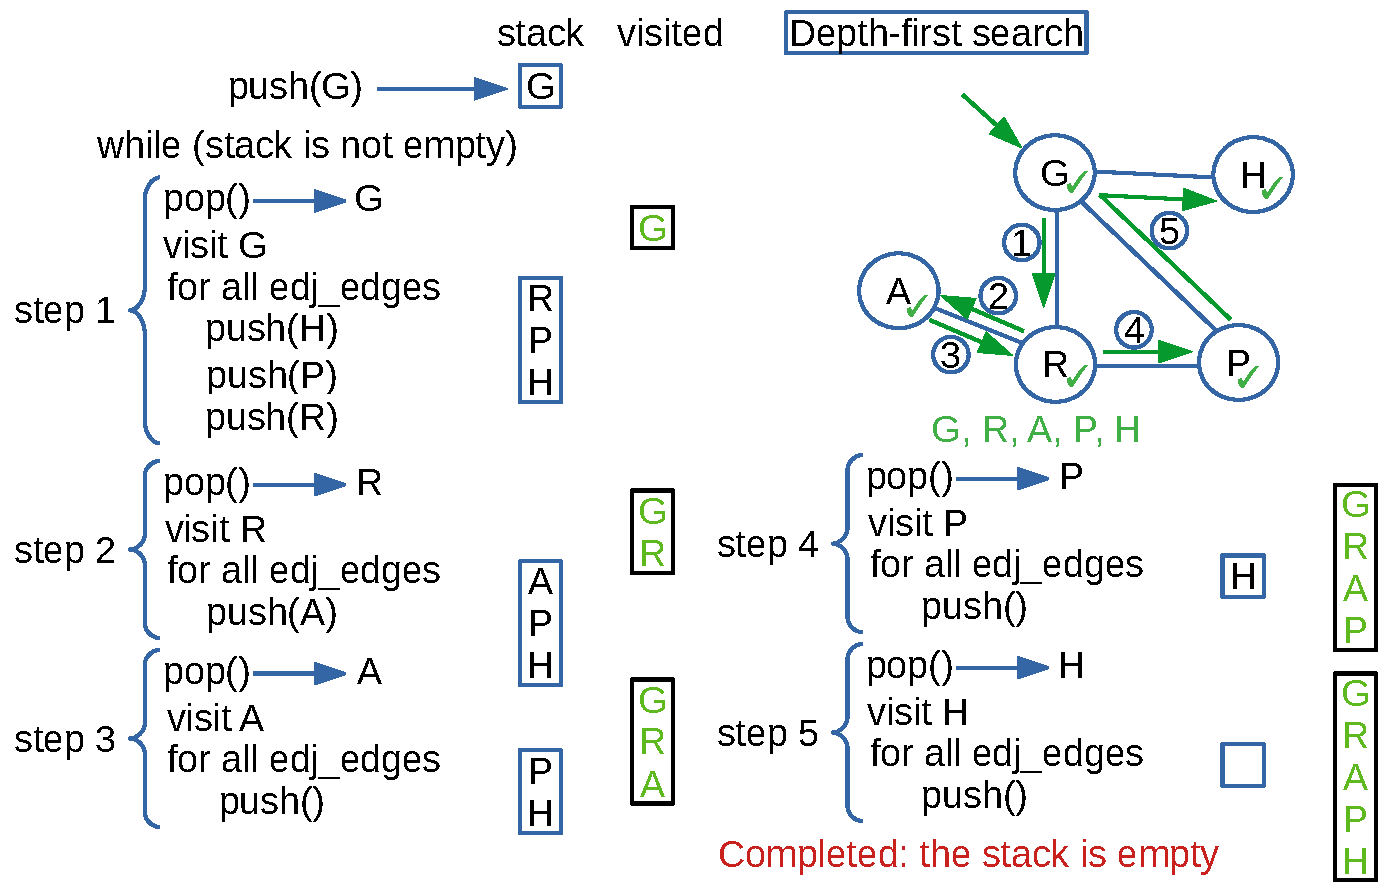
\includegraphics[scale=.6]{/home/omar/Documenti/AlgorithmsNotes/algorithms-notes/chapters/appendix/images/appendixgraphs/graphsappendix_1.pdf}
		\caption[Depth-first search example.]{Depth-first search example.}
		\label{graphappendix_1}
	\end{center}
\end{figure}

\section{Breadth-first search}
In the following there are the pesudocode, the python implementation, and an example of execution of the depth-first search on a graph.

\begin{algorithm}[H]
	\DontPrintSemicolon
	\LinesNumbered
  	\SetKwFunction{FBreadthFirstSearch}{Breadth-first-search}
  	\SetKwProg{Fn}{Function}{:}{}
  	\Fn{\FBreadthFirstSearch{$graph$, $vertex$}}{
		q $\leftarrow$ \textbf{empty queue}\;
		visit(vertex)\;
		q.enqueue(vertex)\;
		\While{\normalfont{\textbf{not} q.isEmpty()}}{
			vertex $\leftarrow$ s.dequeue()\;
			\For{\normalfont{all adjacent nodes adj\textunderscore vertices to vertex}}{
				\If{\normalfont{adj\textunderscore \textbf{not} visited}}{
					visit(adj\textunderscore vertices)\;
					q.enqueue(adj\textunderscore vertices)\;
				}
			}
		}  	
  	}
\caption{Breadth-first search pseudocode.}
\end{algorithm}

\begin{figure}[H]
	\begin{center}
		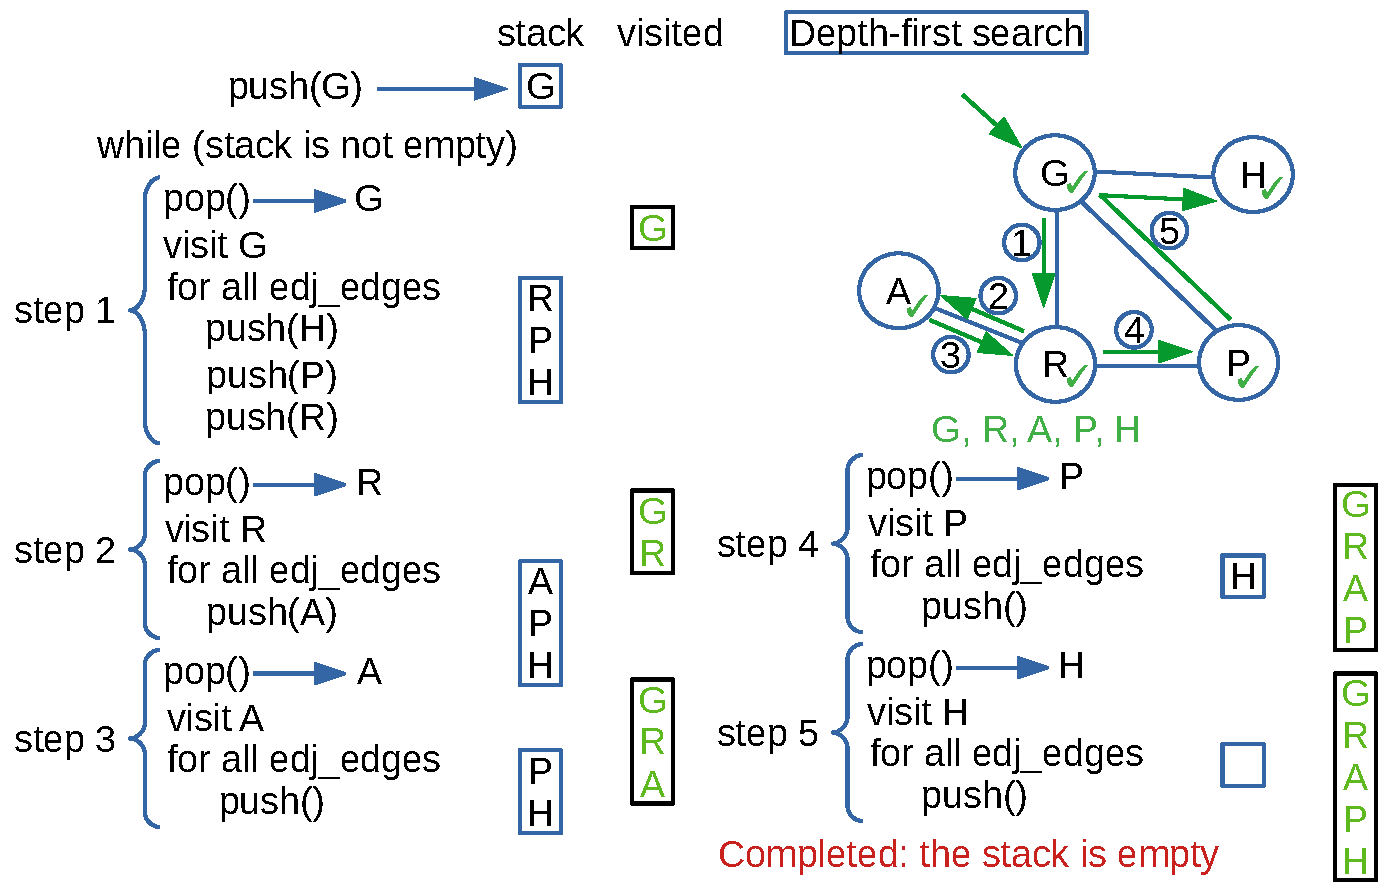
\includegraphics[scale=.6]{/home/omar/Documenti/AlgorithmsNotes/algorithms-notes/chapters/appendix/images/appendixgraphs/graphsappendix_1.pdf}
		\caption[Depth-first search example.]{Depth-first search example.}
		\label{graphappendix_1}
	\end{center}
\end{figure}